\documentclass[10pt]{article}\usepackage[margin=.55in]{geometry}\usepackage[T1]{fontenc}\usepackage{graphicx}\setlength{\parindent}{0pt}\setlength{\parskip}{5pt}\sloppy\begin{document}{\large Private musl gate candidate and native helper checks}\par Task T-1425. 3 November 2026.\par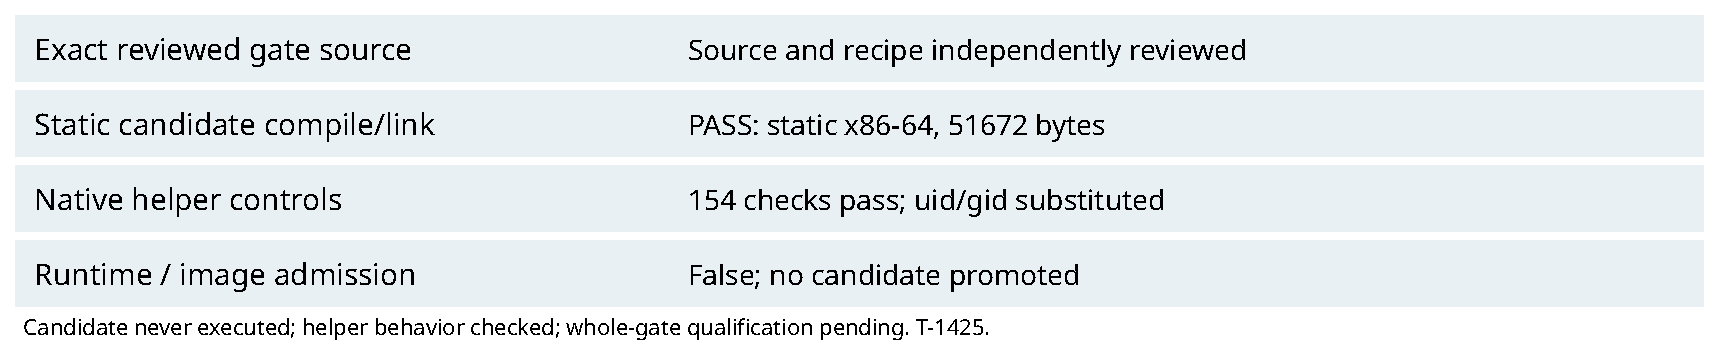
\includegraphics[width=\linewidth]{diagram.pdf}\par The single frozen musl build produced a 51672-byte static x86-64 candidate, SHA256 830406f4c2ddaf900ff4f95ca85f5b1c111b71c9d4d8bf6467ffa46853ae88e9. ELF inspection found no interpreter or needed shared libraries. The candidate was never executed. All 154 native helper checks passed, including 37 partial-file lengths and a real invalid-token timeout of 15.008782 seconds.

The exact reviewed gate source remains 6548d8d41a37975bb30c1a225583113ea6c25056753b3d455d90f1608d8e65bc. All 364 toolchain file hashes and resolved paths were verified before compilation; wrapper, manifest, environment, compiler version/target, commands and resulting binary hashes are retained. The compiler reports x86\_64-amazon-linux; the pinned musl wrapper/specs supply the static libc. The earlier system-GCC static-link failure remains immutable in runtime-private-gate-build.

The frozen outer ceiling was 175 seconds to TERM plus five seconds kill reserve and a 1 GiB address-space limit. Each compile had a 60-second ceiling. The attempt completed in 15.562215 seconds; all six child commands exited zero and were reaped, with no pending signal or uncertain launch. Elapsed time is a validation diagnostic, not a performance comparison.

The helper includes the exact gate source with its main renamed and never invoked. It calls only release\_token and await\_release. Only fstat uid/gid are substituted for unprivileged fixtures; file bytes, mode, type, size and link count are real. Complete tokens, malformed tokens, ownership substitutions, wrong modes, symlink, FIFO, directory, hardlink and bounded waiting are covered. Passing these checks establishes helper behavior under the disclosed substitution; it does not execute the whole gate or validate root ownership, container transport or containment.

A separate non-author reviewer independently checked the frozen recipe and all toolchain pins before execution, then inspected receipt hashes, ELF output, helper stdout and process cleanup. The reviewer executed no binary. Raw receipts and both binaries are archived with official content-addressed transport and fresh remote byte readback. Runtime and image admission remain false. The next concrete dependency is the combined prior parser/gate controls plus held-release controls required by the qualifier receipt contract; this helper receipt is not renamed to satisfy that contract.
\end{document}